\chapter{Collisions} 

The previous sections have neglected the collision operator. 
In this section we describe the collisions as implemented in GKW.  The present implementation neglects the 
finite Larmor radius effects. 
The collisions enter the evolution equation as an additional term 
\begin{equation} 
{\partial \hat{f_a} \over \partial t} = C(\hat{f_a}) .
\end{equation} 
Here we have added the index $a$ to denote the species. 
Useful expressions for the collision operator ($C$) have been published in the literature, usually in the 
($v,\theta$) coordinate system, where $v$ is the velocity and $\theta$ is the pitch angle.
Since the perturbed distribution function is small $f \approx \rho_* F_M$, GKW uses a linearised 
collision operator with the Maxwellian as background. 
This operator has the following form \cite{KAR86} 
\begin{equation} 
C(\hat f_a) = \sum_b {1\over v^2} {\partial \over \partial v} \biggl [ v^2 \biggl ( 
D_{vv}^{a/b} {\partial \hat{f_a} \over \partial v} - F_v^{a/b}\hat{f_a} \biggr ) \biggr ] + {1 \over v 
\sin \theta } {\partial \over \partial \theta} \biggl [ \sin \theta  D_{\theta \theta}^{a/b} 
{1\over v}{\partial \hat{f_a} \over \partial \theta} \biggr ] .
\end{equation} 
Here the sum is over all species $b$. 
$D_{\theta \theta}$ represents the pitch angle scattering, while $D_{vv}$ is the energy scattering
and $F_v$ is the slowing down force. For convenience we split this collision 
operator in three parts 
\begin{equation} 
C(\hat{f}) = C_\theta(\hat{f}) + C_{vv}(\hat{f}) + C_v(\hat{f}),
\end{equation}
where the first part is due to $D_{\theta \theta}$, the second due to $D_{vv}$ and the third 
due to $F_v$. The normalisation of the collision operator follows from the normalisation of the 
gyrokinetic equation as set out in section \ref{sec:normalisation}, giving 
$C_N(\hat{f}_a) = {R_{\rm ref} v_{tha}^3 \over n_a \rho_* v_{\rm thref}} C(\hat{f}_a)$ with the diffusion 
and friction force coefficients made dimensionless accordingly.  

The coefficients can be obtained from the literature \cite{KAR86} (and the references cited therein) and written in normalised form, suppressing the subscript N for the normalised quantities:	
\begin{equation} 
D_{\theta \theta}^{a} = \sum_b {\Gamma^{a/b} \over 4 v_{a}} \biggl [ \biggl ( 2 - {1\over v_{b}^2} \biggr ) 
{\rm erf}(v_{b}) + {1 \over v_{b}} {\rm erf}^\prime (v_{b}) \biggr ] ,
\end{equation}
\begin{equation} 
D_{vv}^{a} = \sum_b { \Gamma^{a/b}  \over 2 v_{a}} \biggl [ {1 \over v_{b}^2} {\rm erf}(v_{b}) - 
{1\over v_{b}}{\rm erf}^\prime (v_{b}) \biggr ] ,
\end{equation} 
\begin{equation} 
F_{v}^{a} = - \sum_b {\Gamma^{a/b} \over v_{a}^2} {m_{Ra} \over m_{Rb}} [ {\rm erf}(v_{b}) - v_{b} {\rm erf}^\prime (v_{b})  ]  .
\end{equation} 
where ${\rm erf}$ is the standard definition of the error function.  The normalised velocity in these equations is defined as 
\begin{equation}
v_{\gamma} =  {v_{Ra} \over v_{R\gamma}}[ v_{\parallel }^2 + 2 \mu B ]^{1/2} ,
\end{equation}
with $\gamma = a$ or $\gamma = b$.  The error function is  
\begin{equation} 
{\rm erf}(u) = {2 \over \sqrt{\pi}} \int_0^u \exp [ -x^2] {\rm d} x 
\end{equation} 
\begin{equation} 
{\rm erf}^\prime(u) = {2 \over \sqrt{\pi}} \exp [ -u^2] 
\end{equation}
Finally the constant $\Gamma^{a/b}$ is given by 
\begin{align} 
\Gamma^{a/b} = {R_{\rm ref} n_b Z_a^2 Z_b^2 e^4 \ln \Lambda^{a/b} \over 4 \pi \epsilon_0^2 m_a^2 v_{tha}^4} = 
6.5141\cdot 10^{-5} {R_{\rm ref} n_{\rm ref}^{19} \over (T_{\rm ref}^k)^2}  {n_{Rb} Z_a^2 Z_b^2 \ln \Lambda^{a/b} 
\over T_{Ra}^2} ,
\label{eq:refquantities-collisions-constraint}
\end{align}
where $R_{\rm ref}$ must be given in meters, $n_{\rm ref}^{19}$ is the reference density in units of $10^{19}$
$m^{-3}$, and $T_{\rm ref}^k$ is the reference temperature in units keV. The Coulomb logarithm is calculated as
\begin{eqnarray}
\ln \Lambda^{e/e} &=& 14.9 - \frac{1}{2}\ln[0.1n_{\rm R}^e n_{\rm ref}^{19}] + \ln[T_{\rm R}^e T_{\rm ref}^k]\\
\ln \Lambda^{e/i} &=& 17.2 - \frac{1}{2}\ln[0.1Z^2n_{\rm R}^e n_{\rm ref}^{19}] + 1.5\ln[T_{\rm R}^e T_{\rm ref}^k] \qquad \textrm{if} \,\, T_e < 10Z^2\,\rm{eV}\\
\ln \Lambda^{e/i} &=& 14.8 - \frac{1}{2}\ln[0.1n_{\rm R}^e n_{\rm ref}^{19}] + \ln[T_{\rm R}^e T_{\rm ref}^k] \qquad \textrm{if} \,\, T_e \geq 10Z^2\,\rm{eV}\\
\ln \Lambda^{i/e} &=& \ln \Lambda^{e/i} \\
\ln \Lambda^{i_1/i_2} &=& 17.3 -\ln[\frac{Z_1Z_2(m_1+m_2)}{m_1T_{\rm R2}T_{\rm ref}^k+m_2T_{\rm R1}T_{\rm ref}^k}] - \frac{1}{2}\ln[0.1\frac{n_{\rm ref}^{19}}{T_{\rm ref}^k}] -\frac{1}{2}\ln[\frac{n_{\rm R1}Z_1^2}{T_{\rm R1}}+\frac{n_{\rm R2}Z_2^2}{T_{\rm R2}}]
\end{eqnarray}
where the superscripts $e$ and $i$ stand for electron and ion, respectively.

Note that the reference density and temperature are defined independently for the collisions and do not need to be equal to the reference density and temperature used in Sec.~\ref{sec:normalisation} for the species parameters. However, the electron density entering the calculation of the Coulomb logarithm is taken to be $n_{\rm R}^e n_{\rm ref}^{19}$ and therefore depends on the normalised electron density given as in an input in the species namelist. The same comments pertains for the temperatures entering the calculation of the Coulomb logarithm.


Using the relation between ($v,\theta$) and the normalised coordinates ($v_{\parallel},\mu$) used in GKW, and performing 
the coordinate transform, one arrives at the explicit expressions given below. The pitch angle scattering term is 
\begin{align}
C_{\theta}  &\rightarrow & 
{2 v_R} {\partial \over \partial v_{\parallel}} \biggl [ {\mu D_{\theta \theta} \over 
v_{\parallel}^2 + 2 \mu B} \biggl ( B {\partial \hat{f}\over \partial v_{\parallel}} - v_{\parallel} 
{\partial \hat{f}\over \partial \mu} \biggr ) \biggr ] \cr 
\noalign{\vskip 0.2 truecm} 
&+& {2 v_R \over  B} {\partial \over \partial \mu} 
\biggl [ {v_{\parallel} \mu D_{\theta \theta} \over v_{\parallel}^2 + 2 \mu B} \biggl ( - B 
{\partial \hat{f} \over \partial v_{\parallel}} + v_{\parallel} {\partial \hat{f}\over \partial \mu} \biggr ) \biggr ] .
\end{align}
The energy scattering yields 
\begin{align}
C_{vv} & \rightarrow & 
v_R {\partial \over \partial v_{\parallel} } 
\biggl [  {v_{\parallel} D_{vv} \over v_{\parallel}^2 + 2 \mu B} \biggl ( v_{\parallel} {\partial 
\hat{f} \over \partial v_{\parallel}} + 2 \mu {\partial \hat{f} \over \partial \mu} \biggr ) \biggr ] \cr 
\noalign{\vskip 0.2 truecm}
&+& v_R {\partial \over \partial \mu} \biggl [ {2 \mu D_{vv} \over v_{\parallel }^2 + 
2 \mu B} \biggl ( v_{\parallel} {\partial \hat{f} \over \partial v_{\parallel}} + 2 \mu {\partial \hat{f} \over 
\partial \mu}\biggr ) \biggr ] .
\end{align}
The slowing down can be written as 
\begin{align}
C_{v}  &\rightarrow & -
v_R {\partial \over \partial v_{\parallel} } \biggl [  {v_{\parallel} F_v \over [ v_{\parallel}^2 
+ 2 \mu B ]^{1/2}} \hat{f}  \biggr ] \cr
\noalign{\vskip 0.2 truecm}
& & - v_R {\partial \over \partial \mu} \biggl [ {2 \mu F_v \over [v_{\parallel }^2 + 
2 \mu B]^{1/2}} \hat{f} \biggr ] . 
\end{align}

The linearised form of the Fokker-Planck collision operator above conserves particle number but does not conserve like particle momentum or 
energy. 
The conservation of parallel momentum and energy can be reintroduced using the following simplified model.  
We are interested in momentum conservation for like particle collisions. 
The change in parallel momentum due to the collision operator above is 
\begin{align}
&& 2 \pi B \int {\rm d}v_\parallel \int {\rm d} \mu v_{\parallel} C(\hat{f}) 
\end{align}
This loss of momentum can be corrected for by adding an ad hoc correction term 
\begin{equation} 
{\partial \hat{f} \over \partial t} = C_{mom} v_{\parallel} F_{M},
\end{equation}
but the energy term isn't simply
\begin{equation} 
{\partial \hat{f} \over \partial t} = C_{ene} (v^{2}_{\parallel} + 2\mu B) F_{M}
\end{equation}
as this would have the effect of adding particles, conservation of which is accounted for by
the differencing and boundary conditions.  Therefore we use
\begin{equation} 
{\partial \hat{f} \over \partial t} = C_{ene}\left( (v^{2}_{\parallel} + 2\mu B) - A\right)F_{M}
\end{equation}
where $A$ is calculated by taking the zeroth moment of the equation
\begin{equation}
\frac{\partial \hat{f}}{\partial t} =  C(\hat{f}) + C_{ene}\left( (v^{2}_{\parallel} + 2\mu B) - A\right)F_{M}
\end{equation}
and setting the change in density to zero.  Since particle conservation is determined by the differencing and boundary conditions, then the coefficient $A$ turns out to be simply:
\begin{equation}
A = \frac{\int {\rm d}v_\parallel \int {\rm d} \mu v^2 F_{M} }{\int {\rm d}v_\parallel \int {\rm d} \mu F_{M}}
\end{equation}
which analytically can be shown to be $\frac{3T}{2}$, but in GKW is calculated numerically to ensure highest precision conservation.

The constant $C_{mom}$ then follows from working out the momentum change due to this term. 
\begin{equation} 
2 \pi B C_{mom} \int {\rm d} v_{\parallel} {\rm d} \mu v_{\parallel}^2 F_{M} +  2 \pi B \int {\rm d}v_\parallel \int {\rm d} \mu v_{\parallel} C(\hat{f}) = 0.
\end{equation} 
while the constant $C_{ene}$ is determined by taking the energy moment $\frac{mv^{2}}{2}$, 
\begin{equation} 
2 \pi B C_{ene} \int {\rm d} v_{\parallel}{\rm d} \mu v^{2}(v^{2}-A) F_{M} +  2 \pi B \int {\rm d}v_\parallel \int {\rm d} \mu (v_{\parallel}^2 + 2\mu B) C(\hat{f}) = 0.
\end{equation}
here we have suppressed the $m/2$ factors as they cancel.

The present form of the collision operator drives the distribution 
towards a Maxwellian with the specified temperature. In the local problem one specifies the temperature as an input 
parameter and no evolution in the temperature is retained. A collision operator that maintains this temperature can therefore 
be considered acceptable.  The steady state distribution function for various velocity space resolutions is plotted in Fig.\ref{maxwellcoll}.

To switch on the conservation terms, which can be switched on or off independently, the parameters
 \name{mom_conservation} $=$  \texttt{.true.} and \name{ene_conservation} $=$  \texttt{.true.}.  However it must be noted that for energy conservation to machine accuracy, the parameter \name{mass_conserve} $=$  \texttt{.true.} must also be set, to enforce conservation at the velocity boundaries (although this may not be the most physical boundary condition).

In GKW the $\mu$-direction grid is non-uniform which represents a problem when differencing the collision terms, however it is
seen that while non-uniform in $\mu$ it is uniform in the $v_{\perp}$ coordinate ($mu = v_{\perp}^2/2B$) and as such the collision operator 
is solved using this as the coordinate as this ensures machine accurate flux conservation and momentum conservation.  To get the collision operator
in this form the following simple transformation must be performed:
\begin{eqnarray}
2{\mu}B &=& v_{\perp}^{2}\\
2\mu\partial/\partial\mu &=& \partial/\partial{v_{\perp}}.
\end{eqnarray} 

\section{Collisions tutorial}

In the previous section we derived the form of the three terms of the Fokker-Plank operator.  
Here we will show, using data produced by GKW and our implementation of the previous to show what effect the operator has on the velocity space structure.

When running GKW, collisions are included if \name{collisions} $=$  \texttt{.true.} in the CONTROL namelist

\subsection{Pitch-angle scattering}

This effect is switched on by setting \name{pitch_angle} $=$ \texttt{.true.} in the collisions input deck.  Pitch-angle scattering conserves momentum and therefore will have the effect of isotropising the distribution function along arcs of constant velocity $v = \sqrt{v_{\parallel}^{2} + 2\mu B}$.  

If we initialise the code with narrow, shifted gaussian in velocity space, then as time progresses then pitch-angle scattering will have the effect of producing a ring in velocity space (As seen in figure \ref{pitch-angle}).

\begin{figure}
\begin{center}
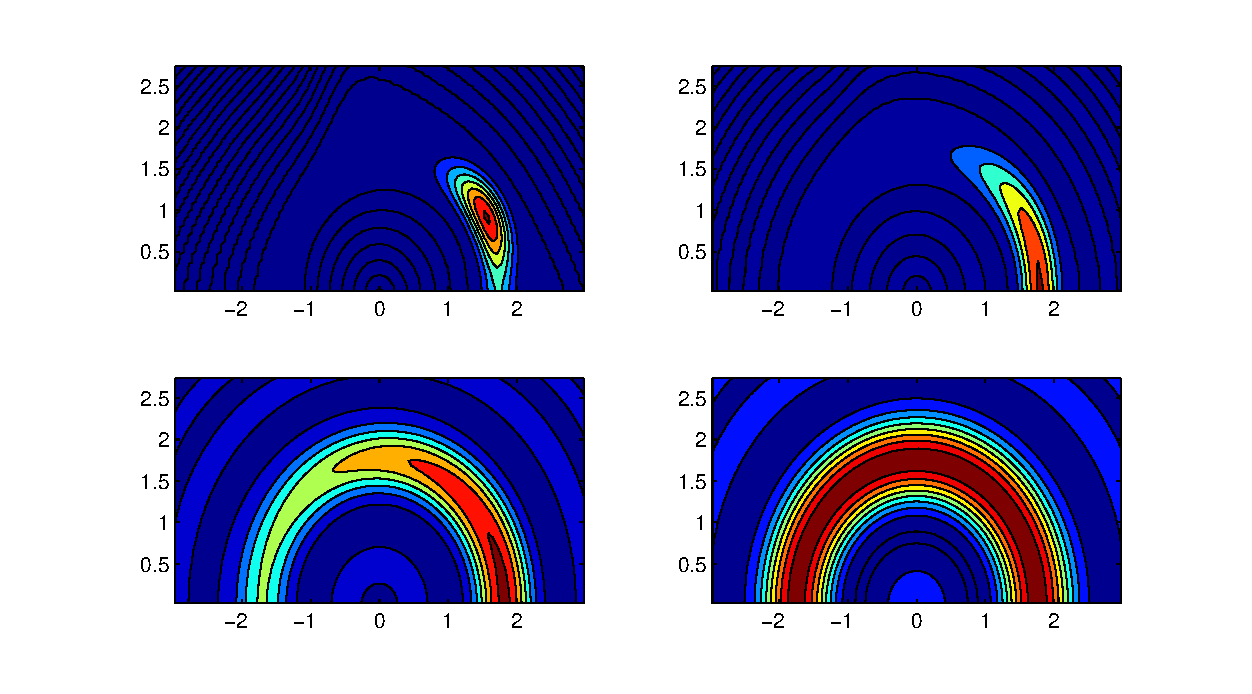
\includegraphics[width=0.6\textwidth]{pitchangle.eps}
\caption{Snapshot of velocity space as three different time intervals showing the effect of pitch angle scattering on the velocity space.  Coordinates are $v_{\parallel}$ horizontally and $v_{\perp}$ vertically. All data shown in this chapter was run with 100 parallel velocity points and 50 $\mu$ points non-equally spaced.\label{pitch-angle}}
\end{center}
\end{figure}

\subsection{Energy scattering}

This effect is switched on by setting \name{en_scatter} $=$ \name{.true.} in the collisions input deck.  The energy scattering term spreads the distribution function in energy.

\subsection{Collisional friction}

This effect is switched on by setting \name{friction_coll} $=$ \name{.true.} in the collisions input deck.  The collisional friction term advects the distribution function towards the origin in velocity space.

When you combine all three effects we get an evolution of the distribution function towards a Maxwellian centred on zero and with a width of a single normalised thermal velocity.

\begin{figure}
\begin{center}
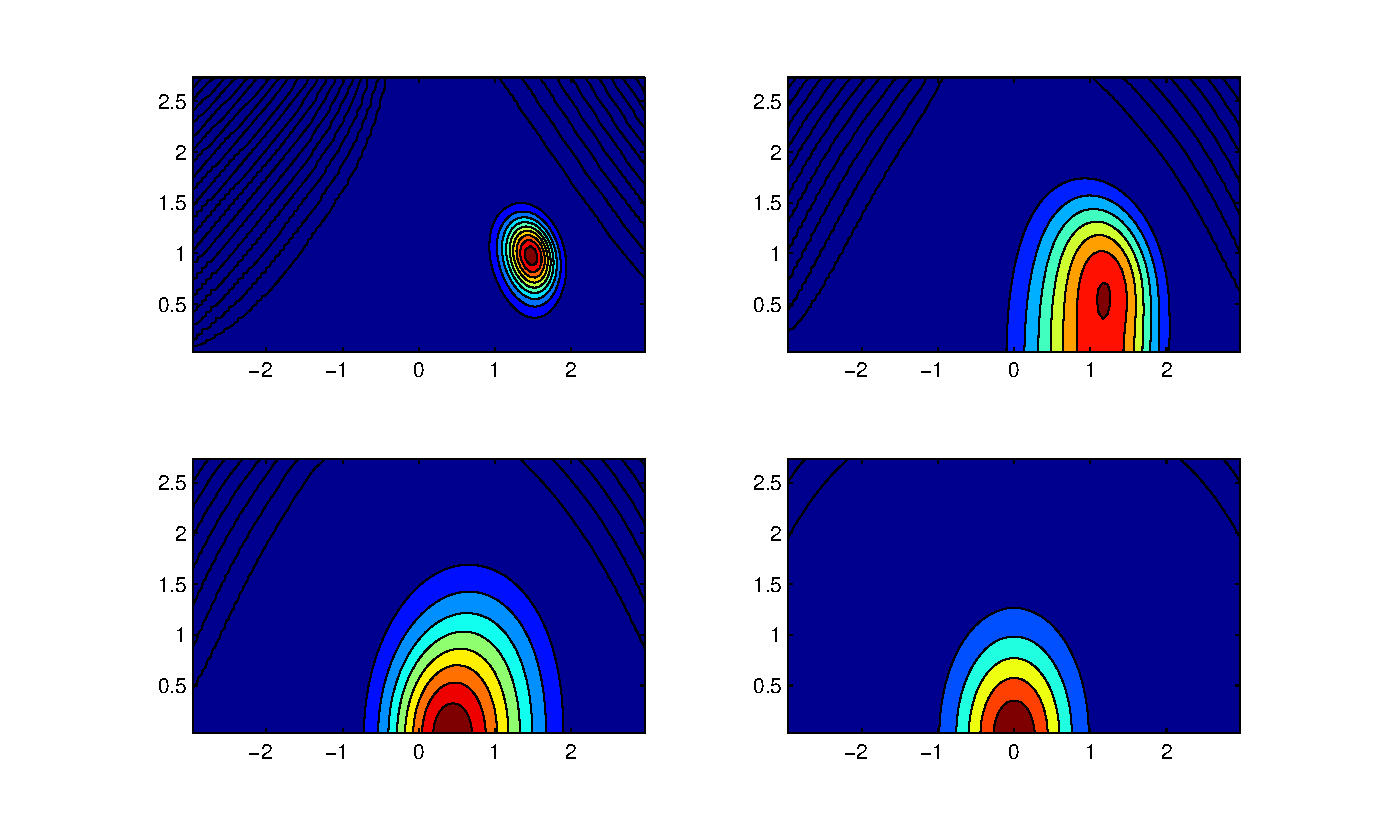
\includegraphics[width=0.6\textwidth]{fulloper.eps}
\caption{Snapshot of velocity space as four different time intervals showing the effect of all the terms in the collision operator on the velocity space.  The final state is a Maxwellian centred on zero.}
\end{center}
\end{figure}

\begin{figure}
\begin{center}
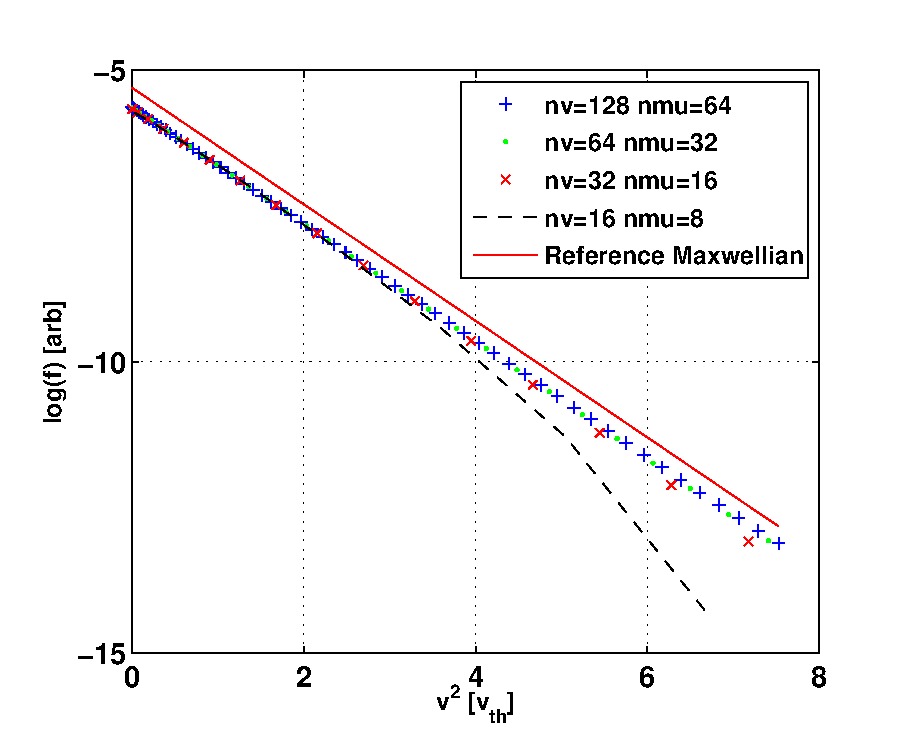
\includegraphics[width=0.65\textwidth]{../benchmarks/collisions/CollisionsMaxwellian.eps}
\caption{Figure showing the logarithm of the distribution function as a function of $v^2$ for varying velocity space resolutions.  A reference 
Maxwellian is also plotted for comparison.}
\label{maxwellcoll}
\end{center}
\end{figure}


\section{Velocity space boundary conditions}

There are currently two options for the boundary conditions in velocity space.  The input deck parameter \name{mass_conserve} changes between open boundary conditions (when set to \texttt{.false.}, default) and zero flux boundary conditions (when set to \texttt{.true.}).  The former is more physical, but the latter is useful for testing of conservation properties to machine precision. The difference in mass conservation between the two is very small.
\begin{figure}
\begin{center}
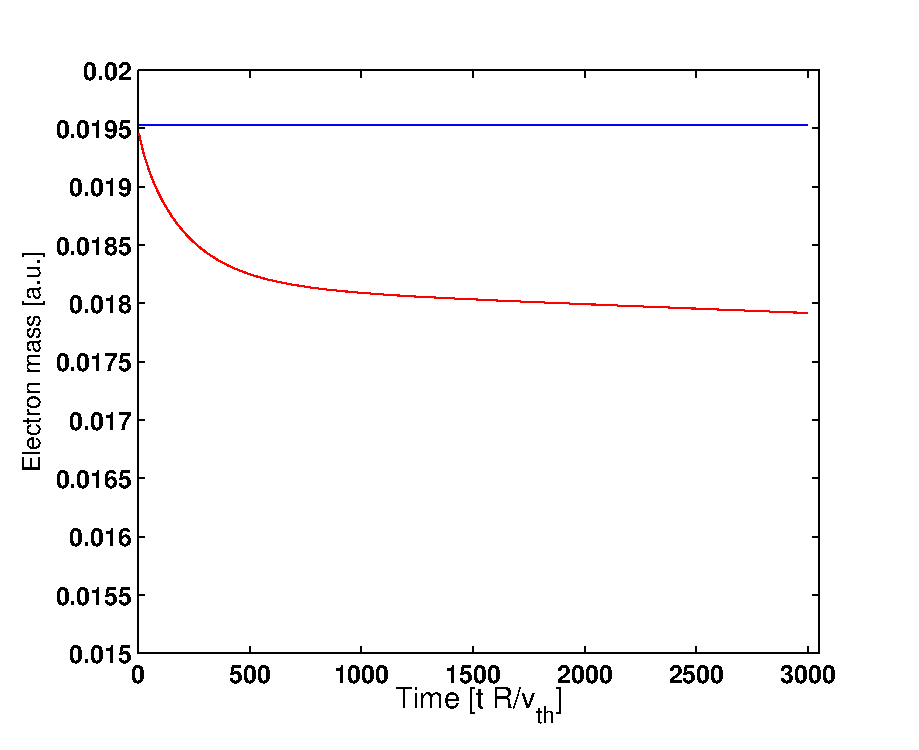
\includegraphics[width=0.45\textwidth]{../benchmarks/collisions/MassConservation.eps}
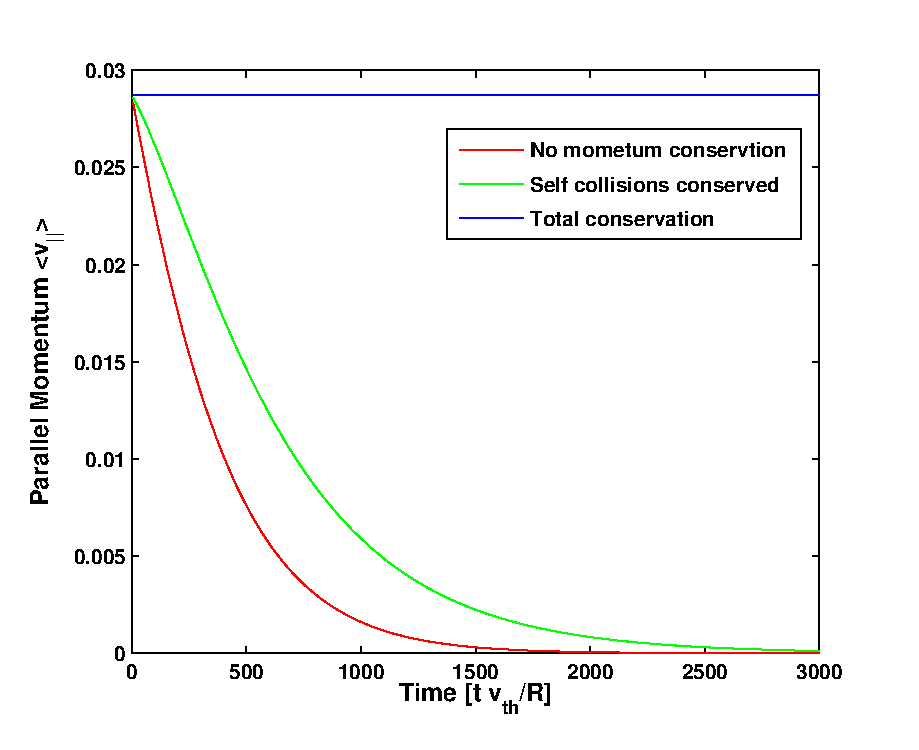
\includegraphics[width=0.45\textwidth]{../benchmarks/collisions/MomentumCons.eps}
\caption{(left) Figure shows the electron particle mass for when (blue) flux conserving boundaries and (red) open boundaries are used.  When the former is chosen the particle number is conserved to machine precision.  
Note the y-axis scale.  (Right) Shows the parallel momentum for runs with the same initial conditions for (blue) fully conservative (green) self collisions conservative
and (red) no conservation at all.  Again, the momentum is conserved to machine precision.  }
\end{center}
\end{figure}

\begin{figure}
\begin{center}
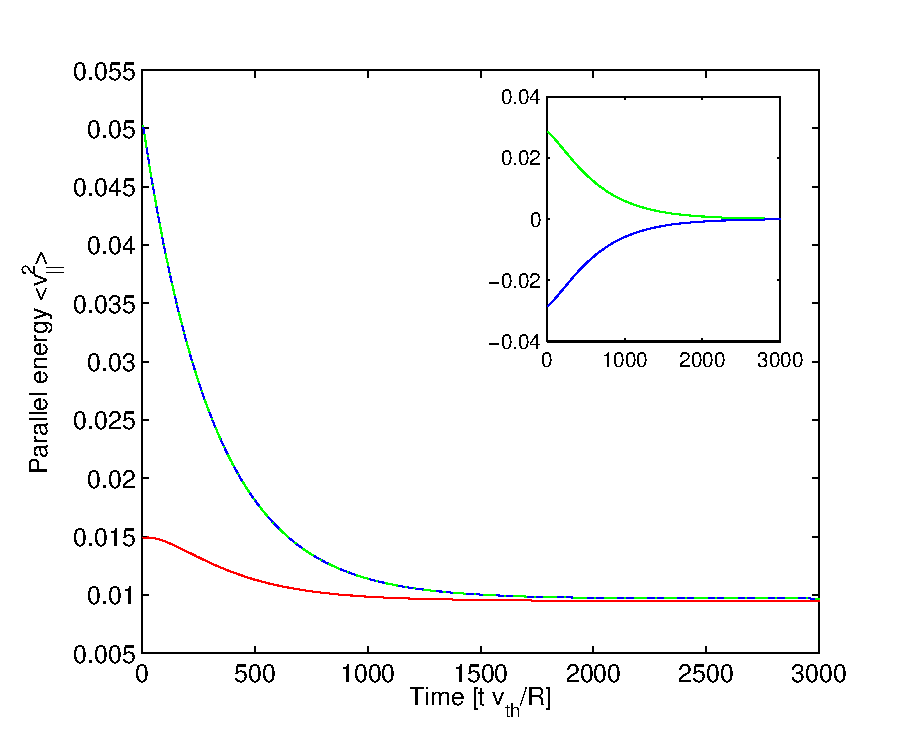
\includegraphics[width=0.5\textwidth]{../benchmarks/collisions/EnergyConvergence.eps}
\caption{Figure shows the energy in the electron distribution for three different initial conditions (green and blue had the same initial width but with a different parallel velocity sign, red was gaussian centered different initial parallel velocity).  
All three converge on the same value. (Inlay is the parallel momentum)}
\end{center}
\end{figure}

\section{User defined collision-frequencies}

The collision frequency can be defined in two ways.  Firstly by specifying \name{nref} which is the particle density in units of $10^{19}$ particles per $m^{3}$, \name{tref}, the temperature in keV and \name{rref} which is the toroidal major radius.  These parameters are what the corresponding parameters are normalised to in the code and are never usually specified.  The normalised collision frequency $\Gamma^{a/b}=\nu_{ab} R_{\rm ref}/v_{\rm tha}$ is given by,

\begin{equation} 
\Gamma^{a/b}_N = {R_{\rm ref} n_b Z_a^2 Z_b^2 e^4 \ln \Lambda^{a/b} \over 4 \pi \epsilon_0^2 m_a^2 v_{tha}^4} = 
6.5141\cdot 10^{-5} {R_{\rm ref} n_{\rm ref}^{19} \over (T_{\rm ref}^k)^2}  {n_{Rb} Z_a^2 Z_b^2 Z^{a/b}_{\rm eff}\ln \Lambda^{a/b} 
\over T_{Ra}^2}
\end{equation}
where $Z^{a/b}_{\rm eff} = 1.0 $ unless $b = i$ (main ion species) as determined by the species density and $a = e$ as determined by the charge on the species.
The value of $Z^{e/i}_{\rm eff}$ is adjusted by the parameter \name{zeff} in the collisions namelist which is 1.0 by default. 
Note that if impurity species are included kinetically, then the scaling factor will be automatically modified to be 
\begin{equation}
 Z^{e/i}_{\rm eff} = 1 + (\name{zeff} - Z_\textrm{eff}^\textrm{sp})\frac{n_e}{n_iZ_i^2}
\end{equation}
with $Z_\textrm{eff}^\textrm{sp}=\frac{1}{n_e}\sum_s n_sZ_s^2$ and the sum on 's' performed on all ion species

However if \name{freq_override} $=$ \texttt{.true.} then,

\begin{equation}
\Gamma^{a/b}_N =  Z_a^2 Z_b^2 \nu_{\rm ref} \frac{n_{Rb}}{T_{Ra}^2} \frac{\ln \Lambda^{a/b}}{\ln \Lambda^{i/i}}
\end{equation}

Where $\nu_{\rm ref}$ is the user defined frequency defined as \name{coll_freq} in the input deck.  This is assumed to be the singly charged ion - ion (proton or deuteron) collision frequency.  To get agreement with the first method this can be set to $6.5141\cdot 10^{-5}R_{\rm ref}n_{\rm ref}^{19}\ln \Lambda^{i/i}/(T_{\rm ref}^k)^2$.  This value is then scaled to all the other species respectively.  For this to work the first species in the input deck should be singly charged ions.

\section{Direct benchmarks}

Here outlined is a direct analytical benchmark of the collision operator. The frictional slowing down of a particle can be calculated 
analytically, and accuratly approximated in the code by using a very narrow, high energy gaussian in velocity space.  The velocity
of this pulse can then be tracked and compared with the analytic expression.

The slowing down time of a particle can be written as:
\begin{equation}
\tau^{s} = - \frac{U}{\frac{\partial U}{\partial t}}
\end{equation}
where $\tau^{s} = 1/\nu_{S}$, which is defined as (we consider only ion-ion collisions):

\begin{equation}
\nu^{a/b}_{S} = - \left[ (1 + \frac{m_{a}}{m_{b}})\psi(x)\right]\nu_{0}^{a/b}
\end{equation}
where $\nu_{0}^{a/b}=\Gamma^{a/b}_N = {R_{\rm ref} n_b Z_a^2 Z_b^2 e^4 \ln \Lambda^{a/b} \over 4 \pi \epsilon_0^2 m_a^2 v_{a}^3} $,
where $\psi(x)$ is the Maxwell integral and can be shown to be $\psi(x) = erf(x) - x \frac{\partial erf(x)}{\partial x}$.  
and x is defined as $v^{a}/v_{th}^{b}$.  This ordinary differential equation can then be solved using standard methods.  The comparison between
GKW and this result is shown in Fig.~\ref{slowdown}.
\begin{figure}[h!]
\begin{center}
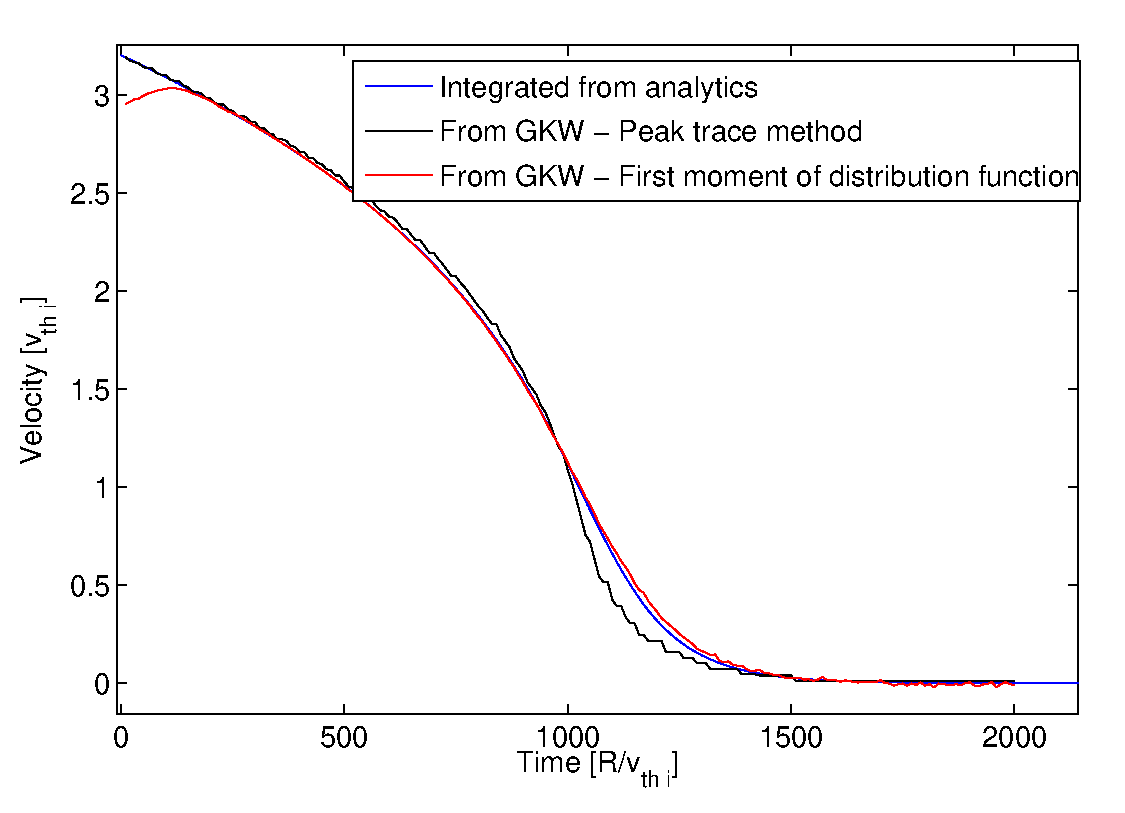
\includegraphics[width=0.60\textwidth]{../benchmarks/collisions/SlowingDownComparison2.eps}
\caption{Measurement of the velocity of a highly localised pulse in velocity space as a function of time.  The result from GKW is shown
utilising two methods, one is the first moment of the distribution function, while the other is simply a trace of the spike.  The blue line is 
the solution of the ODE described above.}
\label{slowdown}
\end{center}
\end{figure} 
Agreement between the two curves is very good, implying that the friction and energy scatter terms are operating correctly
in the current implementation.  A benchmark of the pitch angle scattering against another code is presented in Sec. \ref{linearbenchmarks}.

% related to auctex mode and latex-preview-mode in Emacs:
%%% Local Variables:
%%% mode: latex
%%% TeX-master: "doc"
%%% End:
